\documentclass{ohm_project_description}
\usepackage[english]{babel}

\projecttitle{Drone Charging Setup – Automated Wireless Charging of Micro-Drones}
\projectauthor{Mobile Robotics Lab}
\projectdate{2026}

\begin{document}

\maketitle
\thispagestyle{fancy}

\vspace*{-2.5cm}
\begin{figure}[h!]
    \centering
    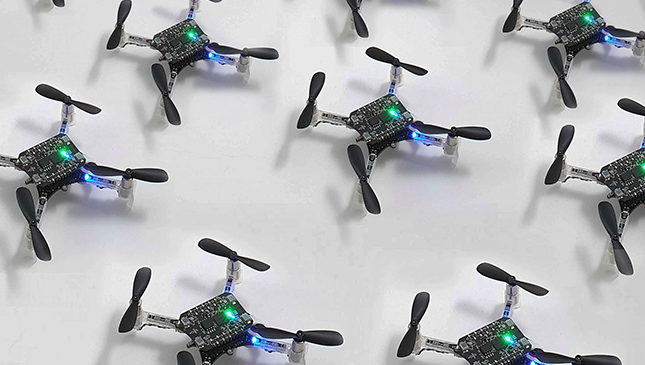
\includegraphics[height=4cm]{img/crazyflies.png}
\end{figure}

A group of Crazyflie micro-drones is now available at the AerodrOHM and can be programmed for coordinated formation flights. For continuous and largely uninterrupted operation of the swarm, a reliable power supply is essential. The goal of this thesis is to develop an automated charging setup in which drones autonomously land on wireless charging pads and recharge there without any manual intervention.

In the first step, a precise approach and landing planning is to be developed that enables the drones to reliably and precisely approach the charging pads. The limited onboard sensors of the drones and the positioning accuracy of the available localisation system must be considered. On the mechanical side, the charging pads are to be designed or adapted to ensure reliable coupling with the drones, potentially involving 3D-printed mounts, guide elements or adapter pieces. Finally, the charging infrastructure is to be integrated into the overall workflow so that the state of charge can be monitored and the transition between flying and charging drones can be automatically coordinated.

\section*{Work Packages}
\begin{itemize}[leftmargin=0.5cm]
    \setlength\itemsep{.1em}
    \item Familiarisation with the drone platform and available charging infrastructure
    \item Development of precise approach and landing planning for the charging pads
    \item Mechanical adaptation and fabrication of components (3D printing)
    \item Integration of the charging infrastructure into the automated workflow
    \item Test and evaluation of the charging setup in the AerodrOHM flight space
\end{itemize}

\section*{Requirements}
\begin{itemize}[leftmargin=0.5cm]
    \setlength\itemsep{.1em}
    \item Programming skills in Python and/or C++
    \item Experience or interest in mechanical design, CAD or prototyping
    \item Enthusiasm for hands-on hardware work and building prototypes
\end{itemize}

\vspace{0.5cm}
This topic can be completed as a \textbf{project, bachelor's or master's thesis} subject to agreement.

\vfill
\textcolor{ohm_red}{\rule{\linewidth}{0.4mm}}
\textbf{\textcolor{ohm_red}{Mobile Robotics Lab}} \\
\begin{tabular}{@{}ll}
\textbf{Supervisor:} & Prof. Dr. Christian Pfitzner \\
\textbf{E-Mail:}     & \href{mailto:christian.pfitzner@th-nuernberg.de}{christian.pfitzner@th-nuernberg.de} \\
\end{tabular}

\end{document}
